\documentclass[8pt]{article}  
\usepackage{latexsym}  
\usepackage[UTF8]{ctex}
\usepackage{geometry}
\geometry{a4paper,left=1.5cm,right=1.5cm,top=1.5cm,bottom=1.5cm}
\usepackage{amsmath}  
\usepackage{amssymb}  
\usepackage{ctex}
\begin{document}  
\zihao{4}
\title{生物智能算法课程报告—协同进化遗传算法 }  
\author { 王雪纯\quad21635075\\数学科学学院}  
\maketitle    
\section{进化计算}  
\vspace{0.1cm}  
\subsection{进化计算的发展}
\begin{description}
        	\item 起源:20世纪50年代,出现最早的关于进化计算的研究报道,其思想是将自然界中的进化思想引入工程研究领域以解决工程中的优化问题。
	\item 发展:20世纪60年代,进化计算得到快速发展,提出了遗传算法和模版理论、进化策略、进化规划。
	\item 成熟:20世纪70年代,标志性事件是Holland于1975年出版著作“Adaptation in Natural and Artificial System”。
	\end{description}
	
\subsection{求解过程(伪代码)}
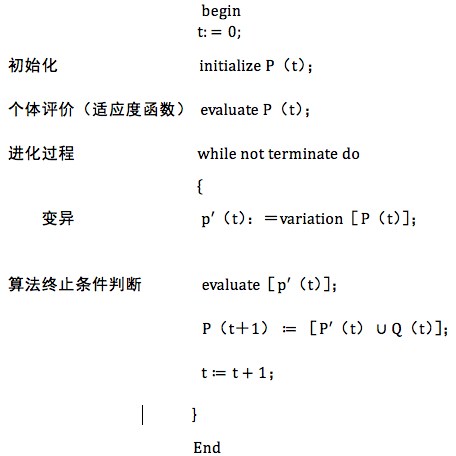
\includegraphics[width=0.59\textwidth]{0.png}

\subsection{进化计算的分类}
        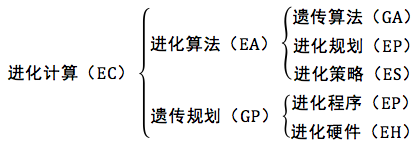
\includegraphics[width=0.54\textwidth]{1.png}
\begin{description}    
        \item (1)进化算法:在进化过程中对某一问题的参数进行优化,优化的结果是某一问题的解。
	\item (2)遗传规划:在进化过程中对能够执行计算的对象进行描述,进化的结果是有关问题的解决过程。
	\end{description}
 \section{协同进化算法}
\subsection{生态学基础}
(1)物种间关系一览表\\\\
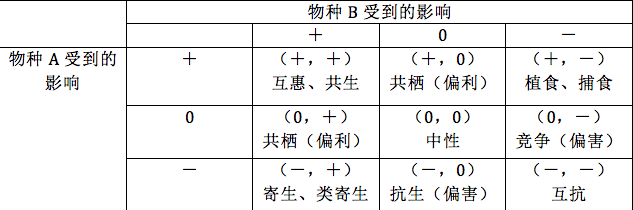
\includegraphics[width=0.8\textwidth]{2.png}\\
\begin{description}
      \item(2)竞争:生活在同一地区的生物个体或种群之间由于资源问题(例如光、水分、食物、空间等)而产生的相互阻碍或制约的负作用,从而影响竞争个体或物种的存活力、生长和繁殖。包括种内竞争和种间竞争。
      \item a.Logistic竞争方程:不考虑种群之间的相互作用,描述了种群内的竞争对整个种群的影响。(k:环境负荷量;r:种群个体增长率;N:种群的大小;(1-N/k):Logistic系数)\\
      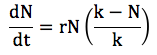
\includegraphics[width=0.2\textwidth]{3.png}      
      \item b.Lotka-Volterra竞争方程:描述了种群内个体之间的竞争以及种群P1和P2之间的竞争。(r1、r2:最大瞬时增长率;aij:竞争系数,表示种群Pj中每个个体对种群Pi的抑制作用)\\
      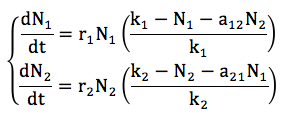
\includegraphics[width=0.4\textwidth]{4.png}
      \item 可能产生的竞争结果:\\
      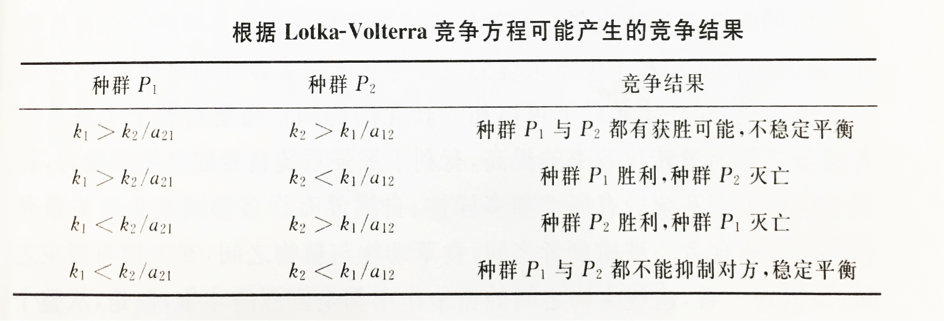
\includegraphics[width=0.85\textwidth]{5.png} \\
      \item 对于一个由n个不同的种群组成的群落:\\     
      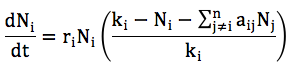
\includegraphics[width=0.37\textwidth]{6.png}\\
      \item(3)协同:生物个体之间既相互竞争,又相互合作,共同收益。例如瞪羚为了不成为猎豹的牺牲品就会越跑越快,但瞪羚提高了奔跑速度反过来又成了作用于猎豹的一种选择压力,促使猎豹也提高奔跑速度。 \\     
      数学模型:\\P:捕食者种群;Q:猎物种群;r1:Q的增长率;r2:P的死亡率;a(常数):P中个体的攻击成功率;b(常数):捕食者将猎物转化为新生捕食者的个体转化率\\
      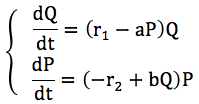
\includegraphics[width=0.24\textwidth]{7.png} \\        
      \item(4)协同进化\\
      a.种群之间性,协同进化存在于种群之间,而不是个体之间;\\
      b.种群性,协同进化存在于两个种群之间,而不是多个种群之间;\\
      c.同时性,种群之间的适应和逆适应是同时发生的;\\
      d.相互性,种群之间的适应和逆适应是相互的。   \\
两种群协同进化示意图:\\\\
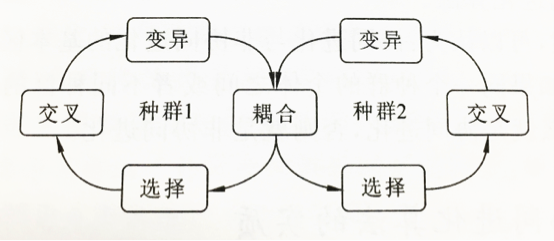
\includegraphics[width=0.65\textwidth]{8.png}
 \end{description}
\subsection{竞争协同进化算法}
\begin{description}
      \item(1)思想:竞争协同进化算法中的个体轮流担任学习者和评价者的角色,轮流给对方施压,轮流刺激对方整体适应度水平的提高。\\
      \item 学习者(L):被计算竞争适应度的个体。
      \item 评价者(E):临时竞争对手。\\
      \item 流程图:\\\\
      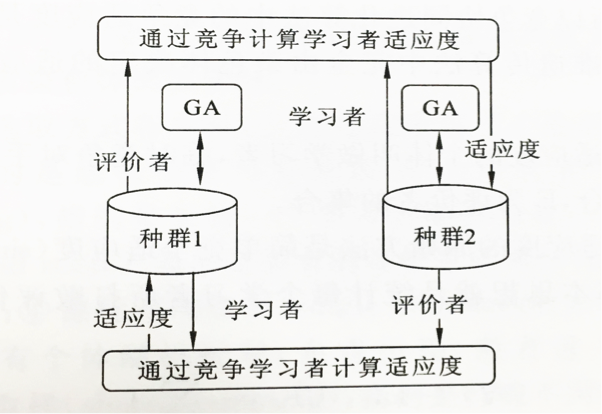
\includegraphics[width=0.65\textwidth]{9.png}
     \item 伪代码:\\
     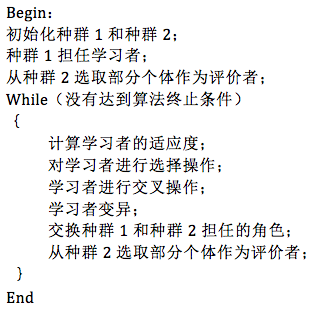
\includegraphics[width=0.55\textwidth]{10.png}     
      \item(2)适应度计算
      \item 竞争适应度:在协同进化算法中的个体适应度,取决于个体临时竞争对手在竞争当中的表现。其基本思想是统计每个学习者打败评估者的次数。
      \item 常用方法:共享竞争适应度\\
      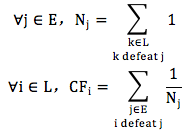
\includegraphics[width=0.35\textwidth]{11.png}    \\
      (对于某个评价者j,有Nj个学习者可以将其打败,考虑每个学习者适应度的贡献比例为1/Nj;对于某个学习者i,其共享竞争适应度为对它能够打败的每个评价者的贡献比例进行求和)    
        \item(3)优点
        \item a.竞争协同进化算法不仅模拟了达尔文进化论中的适者生存、优胜劣汰现象,还模拟了生态系统中普遍存在的协同进化现象,是对自然界中的生态进化的一种更准确的模拟。
        \item b.竞争协同进化算法不仅能够通过生存的压力(由选择算子来实现)提高群体总的适应度,而且能够鼓励新颖积木块的出现,从而维护群体的多样性,这样有助于解决标准遗传算法中长期存在的过早收敛的问题。   
        \item c.竞争协同进化算法中的竞争适应度是由个体在竞争中的表现来决定的,所以当由染色体决定的绝对适应度无法直接有效地定义时,竞争协同进化算法的优势就尤为明显。        
        \item(4)弊端\\
       a.转圈。在竞争协同进化算法中,个体适应度的评价依据是个体在竞争中是否取胜、是否战胜对手。个体进化的目的是打败对手,而不是在保留以前进化的基础上进一步进化,这样可能导致以前进化中的优良积木块的丢失,从而可能出现“形成优良积木块-丢失优良积木块-形成优良积木块-丢失优良积木块”这样的一个转圈弊端。其他一些效果也可能导致转圈的出现,如锤子-剪刀-布等不可传递的优越关系、重复的军备竞赛。\\
改进策略:最佳个体保留策略等。\\
       b.脱节。当评价者全部被打败或者全部无法被打败时,学习者的适应度多样性趋近于零,那么选择梯度就会消失,无法形成一种你追我赶的军备竞赛。改进策略:建立测试银行、“友善竞争者”等。\\
       c.过度集中.个体进化的压力和动力是打败对手,如果对手的多样性不够,那么那么最后进化的结果就没有普遍适应性,不是能够打败所有可能对手的最优个体,而是只能打败部分对手的局部最优个体。\\        
        \item(5)应用\\
        \item a.排序网的设计:排序网的功能是对输入数据排序,一般根据输入数据的多少进行划分。排序网的性能由“比较-交换”的次数决定,次数越少的排序网的性能越优,对于相同类型的排序网,“比较-交换”的次数越少,那么所需的时间也越少。Hillis于1990年首次把捕食现象作为计算模型引入计算科学,将一种寄生物和宿主协同进化的机制应用到优化搜索的改进中,提出了协同进化遗传算法,采用多种群的方式实现竞争协同进化算法中,成功地解决了16输入排序网的设计。        
        \item b.博弈游戏:协同进化算法具有博弈论背景,很自然地进行协同进化算法可以应用到带博弈论色彩的游戏中,特别是“零和博弈”游戏中。例如,井字游戏、拿字游戏、囚徒困境、追逃等游戏,在这些游戏中,一方胜利意味着另一方失败。一些研究竞争协同进化算法的学者常拿这些游戏作为算法的测试对象。              
        \item c.模式识别:Kowaliw等人在开发自动模式识别软件CellNet的过程中,加入了竞争协同进化,开发了一个称为CellNet Co-Ev的版本,在CellNet Co-Ev中,识别器被看成捕食者,而模式被看成是猎物,识别器与模式通过竞争的方式协同进化。        
        \item d.作业调度: 网格由多个高性能计算中心组成,用户向本地的HPC提交作业,网格的作业调度系统确定这项作业是在本地的HPC中心执行还是在异地的HPC中心执行。在一个网格中,理想的调度结果是作业平均地分配在不同的HPC中心,但是每个HPC中心都倾向于本地的相应时间最短。所以,网格所采用的作业调度策略非常重要。        
	\end{description}
\subsection{合作协同进化算法}
\begin{description}
      \item(1)思想:传统的遗传算法中只有一个种群在进化,种群中的每一个个体表示一个完整的解,而合作协同进化算法包含处于合作关系的多个种群同时进化,种群中的每一个个体只表示解的一部分。例如一个包含三个子群体的合作协同进化算法子群体中的个体相对独立地通过选择、交叉、变异等算子发生进化,每个群体中的个体都只是表示完整解的一部分,来自三个种群中的个体只有合作,才能组成一个完整解。三个子群体中的个体通过共享的领域模型发生合作关系。
      \item 种群纵向划分示意图:\\\\
       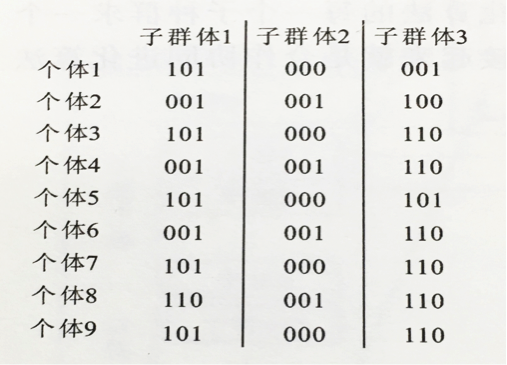
\includegraphics[width=0.65\textwidth]{12.png}
      \item 伪代码:\\
      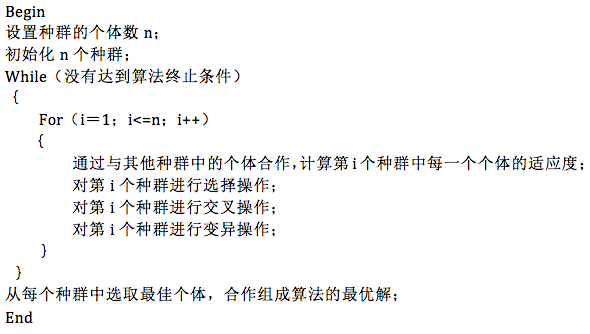
\includegraphics[width=0.95\textwidth]{13.png}
      \item 合作协同进化算法拓扑模型图:\\
      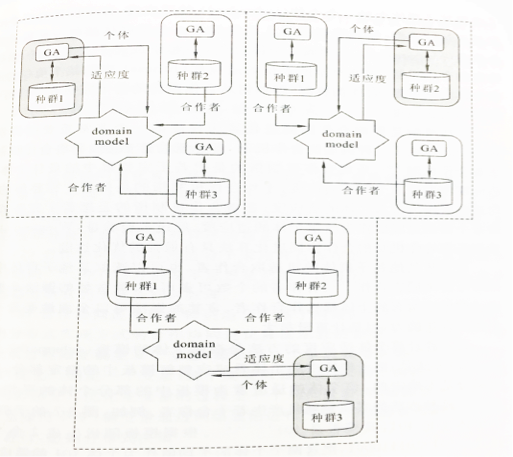
\includegraphics[width=0.6\textwidth]{14.png}
        \item(2)适应度计算\\
        个体适应度表现为与其他各子群体中的个体的合作能力。为了求得某子群体中的一个个体的适应度,该子群体先把个体发送至领域模型(domain model),领域模型同时接收一定数量的合作者来同那个个体合作,一起组成若干完整解,根据特定的合作机制,在领域模型中完成所有个体适应度的计算。
        \item 合作机制:即如何从若干完整解中得到所求个体的适应度。如乐观合作机制(取最佳)、平均合作机制(取平均)、悲观合作机制(取最差)等。
        \item 随机产生若干合作者:把子群体中的个体看成完整模版解中的确定部分,而其他部分是不确定的,该个体的适应度为模版中的部分个体的平均适应度。
      \item(3)优点:
      \item a.合作协同算法采用分而治之、分工合作的思想,特别适合于解决现实生活中的大规模非线性问题。
      \item b.合作协同算法适合于采用并行程序的方式实现,从而减少运行时间。
      \item c.合作协同算法特别适合于基于网络的分布式决策和规划。    
      \item(4)弊端:
      \item a.个体适应度的准确性问题。对于同一个个体,如果合作者不一样,得到的适应度会不一样。
      \item b.适应度计算过程中减少计算量和减少偶然性无法兼得。选取的合作者的个数越少,计算个体的适应度的偶然性就越大;选取的合作者的个数越多,计算量就越大。
      \item(5)应用\\
      \item a.人工神经网络:Garcia-Pedrajas采用合作协同进化算法成功设计了高性能的神经网络集成器。各神经网络不是单独设计,而是采用多目标的方式,鼓励各神经网络之间的合作。各神经网络既需要考虑在给定问题上的性能,又需考虑同其他神经网络的合作。在probenl测试集以及10个实际分类问题上的测试结果表明:Garcia-Pedrajas采用合作协同进化算法设计所得的神经网络集成器具有较好的性能。
      \item b.计算机视觉:Krawiec K.把合作协同进化算法成功地应用到计算机视觉中,把计算机视觉学习的复杂度通过合作协同进化算法实现了基因级别的自动分解,对输入图像采取的一系列特征提取操作和计算机视觉操作协同工作,在实际合成孔雷达的三维目标识别中取得了良好的检测效果。
      \item c.多目标优化:Tan等采用分而治之的策略,采用合作协同进化算法来解决多目标优化。多目标优化试验结果表明CCEA能够有效地保持种群的多样性,并把解均匀地分布在Pareto前沿。Tan等用主从模式的并行处理器实现了分布式的合作协同进化算法(DCCEA),DCCEA在保持CCEA的搜索性能的前提下,减少了时间消耗。      
      \item d.作业调度:Kim提出一种共生进化算法,采用局部相互作用、稳态复制策略,随机选择合作者(即共生体),同时有效地解决了生产过程中的过程规划和作业调度这俩个互相联系的问题。      
      \item e.价格跟踪:郑浩然等提出一种多模式共生进化算法(MSEA),借鉴生物在生态环境中对某一特定环境压力的多策略机制,成功地应用到了价格跟踪体系中。在MSEA中,每一个共生体表示一个部分解,随机选取合作者来计算共生体的适应度,选取10次的平均值作为所取共生体的适应度。      
      \item f.卫星舱布局设计:卫星舱布局设计是一个复杂的耦合问题,也是一个组合优化问题,很容易导致局部最优。Teng与Chen等在SMLD中再用分而治之的策略,根据卫星舱的物理结构,把复杂的SMLD分解为容易处理的子系统设计,采用合作协同进化算法进行工程优化,达到了缓解局部最优的目的。      
      \end{description}  
\end{document}   